\documentclass[12pt,letterpaper,noanswers]{exam}
\usepackage[usenames,dvipsnames,svgnames,table]{xcolor}
\usepackage[margin=0.9in]{geometry}
\renewcommand{\familydefault}{\sfdefault}
\usepackage{multicol}
\pagestyle{head}
\header{AM 111 Class 11}{}{Numerical differentiation, p.\thepage}
\runningheadrule
\headrule
\usepackage{siunitx}
\usepackage{graphicx} % more modern
\usepackage{amsmath} 
\usepackage{amssymb} 
\usepackage{hyperref}
\usepackage{tcolorbox}
\usepackage{enumitem}
\def\mbf{\mathbf}
\newcommand{\vc}[1]{\boldsymbol{#1}}
\def\dsst{\displaystyle}
\DeclareMathOperator*{\argmin}{arg\,min} % thin space, limits underneath in displays


\begin{document}
 \pdfpageheight 11in 
  \pdfpagewidth 8.5in

\noindent 

\section*{Preliminaries}

\begin{itemize}
\itemsep0pt
\item The problem set is due on Friday at 5pm (submit via Gradescope: include pdfs of all code/output on Gradescope.  Upload any source code to Canvas).  If you are using an extension, the deadline is Sunday at 5pm to receive feedback on your work before the quiz.
\item If you need guidance, help, or suggestions on the problem set, post to Ed.
\item There will be a skill check in class during the next class.  The problem info is below.
\item There is a pre-class assignment for Class 12 (Tuesday).  See Canvas.
\item Quiz info is on Canvas.
\item There is no problem set next week (quiz instead).
\end{itemize}


\noindent\textbf{Big picture}

Today: Approximating $\frac{df}{dx}$ at a point $x_0$.

\vspace{0.2cm}
\hrule
\vspace{0.2cm}

\noindent \textbf{Skill check practice}
\begin{questions}
\item Let $f(x) = x^3 - 3x$.  Write an expression for $f'(x)$ approximated using central differences at $x_0 = 2.0$ with $h = 0.01$.

\emph{You will be asked for one of forward differences, central differences, or backward differences.}


\item The skill from the Class 08 handout (Skill Check C09).
\end{questions}


\vspace{0.2cm}
\hrule
\vspace{0.2cm}

\noindent \textbf{Skill check solution}
\begin{questions}
\item The formula is $(f(x+h) - f(x-h))/(2h)$ so $\dfrac{2.01^3-3*2.01 - 2^3+3*2}{0.02}$.

\item See the past handout.
\end{questions}
\vspace{0.2cm}
\hrule
\vspace{0.2cm}

\noindent \textbf{Teams}
\begin{multicols}{3}
1. Eletria, Benjamin, Marissa

2. Cameron, Basil, Emma

3. RH, Eric, Esmé

4. Nini, Ray, Dani

5. Jack, Mina, Ivonne

6. Alex, KevinG, Shang

7. Jessica, Johan, Tom

8. Nina, Robert, Padraig

9. KevinC, Alex, Eli

10.  Aidan, Daniyal, Zachary

11. JuliaK, JuliaM

12. Mack, Brian

13. Caitlin, Sophie

\end{multicols}

\section*{Numerical differentiation}

(Sauer \S 5)

\noindent Application 1: Given a function, $f(x)$, in closed form, find the derivative of $f$ at a point $x = x_0$. 

\noindent Application 2: Given a function, $f(x)$, where the output can be found (via a computer simulation, an experiment, or otherwise), approximate $\dfrac{df}{dx}$ at a point $x = x_0$.

\noindent Application 3: Given a set of values $\{(x_i,y_i)\}_{i=1}^N$, treat $y$ as the output of a function, $f(x)$, and estimate $\dfrac{df}{dx}$ at a point $x = x_0$.

\eject

\noindent\textbf{Symbolic derivatives}
\begin{tcolorbox}

(Humpherys Volume 1 Lab 8)

To take the derivatives of a function known in closed form, try symbolic differentiation.  In Python the package is \texttt{sympy}.
\begin{verbatim}
import sympy as sy
x = sy.symbols('x')
# Differentiate x^3 + x with respect to x:
sy.diff(x**3 + x, x)
\end{verbatim}

You can evaluate the output of \texttt{sy.diff} at a point $x_0$ to find a value for $f'(x_0)$.
\end{tcolorbox}

\noindent\textbf{Approximating derivatives via finite differences}
\begin{tcolorbox}

(Sauer \S 5.1.1)

\[\frac{df}{dx} = \lim\limits_{h\rightarrow 0} \frac{f(x+h)-f(x)}{h}\]

For $f$ twice differentiable, Taylor's theorem says
\[f(x+h) = f(x) + hf'(x) + \frac{1}{2}h^2 f''(c)\] where $x< c< x+h$.
\end{tcolorbox}
\begin{enumerate}[resume=classQ]
\item Rearrange the expression above from Taylor's theorem to isolate $f'(x)$ on the left hand side.
\vspace{1in}

\end{enumerate}

\begin{tcolorbox}
\begin{itemize}
\itemsep0pt
    \item The two point \textbf{forward difference} formula, $f'(x)\approx \dfrac{f(x+h)-f(x)}{h}$ is a first order method for approximating $f'(x)$.
    \item The two point \textbf{backward difference} formula, $f'(x)\approx \dfrac{f(x)-f(x-h)}{h}$ is also a first order method for approximating $f'(x)$.
    \item This type of method is most useful when you are able to choose the evaluation values for the function (so Application 1 or Application 2 above).
    \item When the error for a method of $\mathcal{O}(h^n)$ the method is referred to as \textbf{order} $n$.
    \item For a first order method, cutting $h$ in half should cut the error approximately in half.
    \item The error in the method found using Taylor's theorem is called \textbf{truncation error} or \textbf{discretization error}.
\end{itemize}
\end{tcolorbox}

\begin{enumerate}[resume=classQ]
\item The three point \textbf{centered difference} formula is given by $f'(x) \approx \dfrac{f(x+h)-f(x-h)}{2h}$.  We want to find the truncation error.
\begin{parts}
\item Taylor expand $f(x+h)$ and $f(x-h)$ to second order as was done for the forward difference formula.  When you calculate $\dfrac{f(x+h)-f(x-h)}{2h}$ what do you find?
\vspace{1in}

\item Find $n$ such that $f'(x) = \dfrac{f(x+h)-f(x-h)}{2h} + h^n k$ where $k$ is a constant.
\vspace{1cm}

\end{parts}
\end{enumerate}
\begin{tcolorbox}
(Sauer \S 5.1.2)

$f(x-h)$, $f(x)$, and $f(x+h)$ are nearly equal numbers.  In floating point arithmetic, subtracting nearly equal numbers can lead to roundoff error.
\end{tcolorbox}
\begin{enumerate}[resume=classQ]
\item Let the floating point version of $f(x+h)$ be $\hat{f}(x+h)$.

$\hat{f}(x+h) = f(x+h) + \epsilon_1$ where $\vert \epsilon_1\vert \approx \epsilon_{\text{mach}}$.

$\hat{f}(x) = f(x) + \epsilon_2$ where $\vert \epsilon_2\vert \approx \epsilon_{\text{mach}}$.

$\hat{f}(x-h) = f(x-h) + \epsilon_3$ where $\vert \epsilon_3\vert \approx \epsilon_{\text{mach}}$.

\begin{parts}
\item Compare $\dfrac{\hat{f}(x+h) - \hat{f}(x)}{h}$ to $\dfrac{f(x+h) - f(x)}{h}$.  What is the maximum error due to rounding?
\vspace{1in}

\item Sum the truncation error and the rounding error to generate an error estimate for $f'(x)$ when calculated using forward differences.
\vspace{1cm}


\item Do the same for $f'(x)$ when calculated using central differences.
\vspace{1in}

\end{parts}


\end{enumerate}

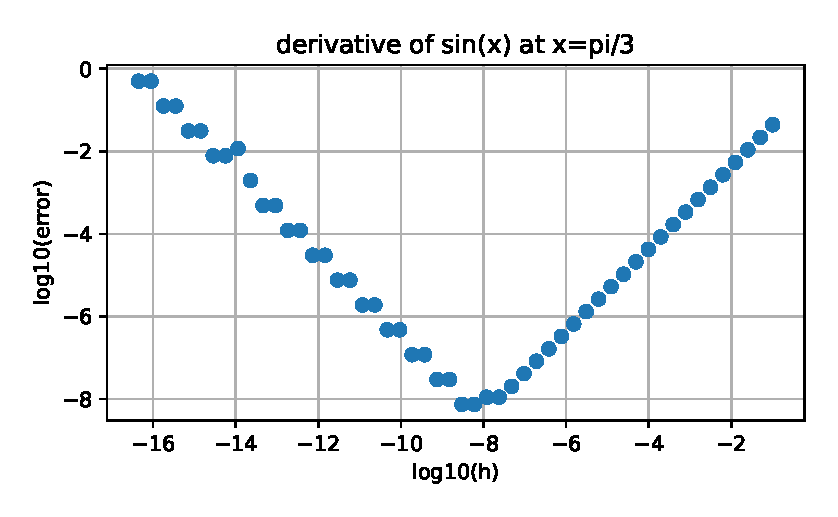
\includegraphics[width=0.5\textwidth]{img/Class11sinforward.eps}


\begin{enumerate}[resume=classQ]
\item Examine the log-log plot of error shown above.
\begin{parts}
\item The error function is approximately two straight lines on the log-log plot.  Which part is dominated by truncation error and which by rounding error?
\vspace{1cm}

\item Using the grid, approximate the two slopes.
\vspace{1cm}

\item Which error function do they match?  Take the log of both sides of your error function to identify the expected slopes.
\vspace{1in}

\item Answer the same questions for the plot below.
\vspace{1in}

\end{parts}

\end{enumerate}


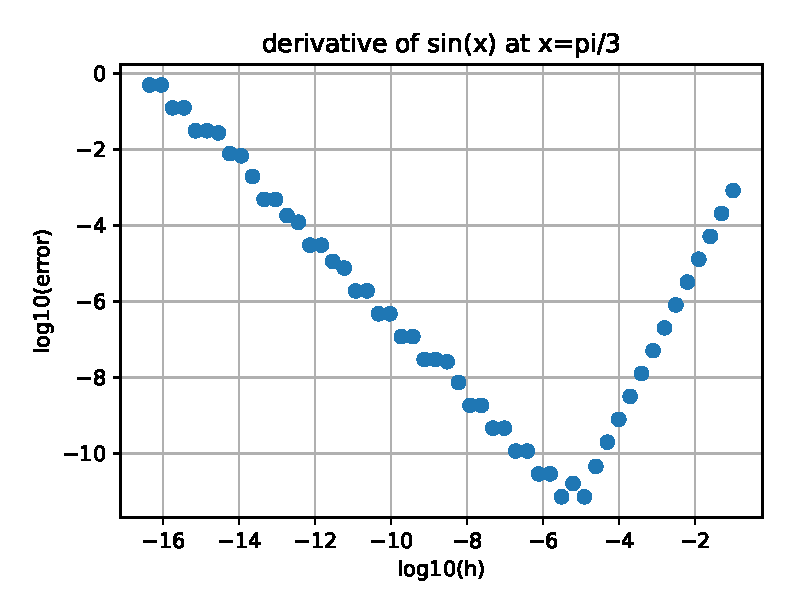
\includegraphics[width=0.45\textwidth]{img/Class11sincentral.eps}

\begin{enumerate}[resume=classQ]
\item For each error function, find the minimum value of $h$ in terms of machine epsilon.

Compare your findings to the plots.
\vspace{1in}
\end{enumerate}

\noindent\textbf{Approximating a derivative from data}
\begin{tcolorbox}
(Greenbaum and Chartier \S 9.1)

Application 3: Given a set of values $\{(x_i,y_i)\}_{i=1}^N$, treat $y$ as the output of a function, $f(x)$, and estimate $\dfrac{df}{dx}$ at a point $x = x_0$.
\begin{itemize}
\itemsep0pt
    \item The value $y_i$ has an associated measurement error (it is not exactly $f(x_i)$.
    \item These errors will be much larger than $\epsilon_{\text{mach}}$
\end{itemize}
\end{tcolorbox}
\begin{enumerate}[resume=classQ]
\item Assume the maximum measurement error is $\delta \vert f(x_i)\vert$.  Replace $\epsilon_{\text{mach}}$ in your rounding error calculation with $\delta \vert f(x_i)\vert$ to find an expression for the maximum error due to measurement error.

\vspace{1in}


%then it propagates to the derivative as $\dfrac{\delta}{h}(\vert f(x_{i+1})\vert + \vert f(x_{i})\vert)$ where $h = x_{i+1}-x_i$.
\end{enumerate}

\begin{tcolorbox}

It can be difficult (or impossible) to choose a spacing to the data that balances truncation error with measurement error.  Approximating a derivative from data using finite differences may \textbf{not} be possible.

\begin{itemize}
\itemsep0pt
    \item Additional option: find an interpolating function and take the derivative of that.
    \item Additional option: fit a function to the data (linear least squares or another fitting method) and take the derivative of that.
\end{itemize}

Major caveat: Two functions can have very similar values on an interval while having very different derivatives.  
\end{tcolorbox}
\begin{enumerate}[resume=classQ]
\item Consider the three functions plotted on the left below.  
\begin{parts}
\item What is the largest difference in $y$ that occurs between any two functions?  What is the smallest difference?
\vspace{1cm}
\item Find the derivative of each function.
\vspace{1in}
\item If the true function were $f(x) = x$, but your measurement method added high frequency noise, so that the data looked exactly like $x + 0.01\sin(100x)$, what is the maximum error you would see in the derivative?
\vspace{1cm}

\item Thinking of your derivative as your output (forward error) and your measurements as your input (backward error), create an estimate of an absolute condition number.
\vspace{1cm}
\end{parts}



\end{enumerate}

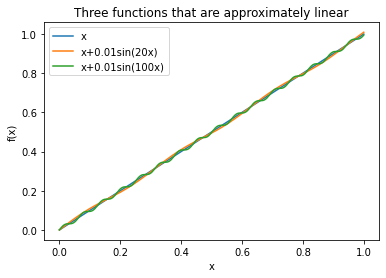
\includegraphics[width = 0.45\linewidth]{img/Class11lines.png}
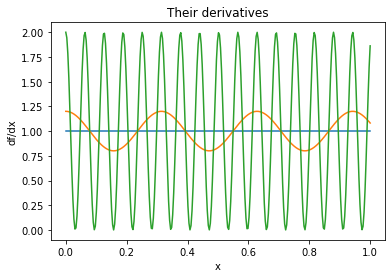
\includegraphics[width = 0.45\linewidth]{img/Class11linederiv.png}

% \begin{enumerate}[resume=classQ]
% \item 
% \end{enumerate}

\begin{tcolorbox}

Without additional information or assumptions about the structure of $f(x)$ (including information that constrains the 2nd or 3rd derivative), it may not be possible for the problem of estimating a derivative from data to be well-posed.

\begin{itemize}
\itemsep0pt
    \item A \textbf{well-posed problem} is one where a solution exists and is unique, and the behavior of the solution changes continuously with change in the initial conditions.  \url{https://en.wikipedia.org/wiki/Well-posed_problem}
    \item In an \textbf{ill-posed problem}, some aspect of well-posedness is violated: the solution might not exist; it might not be unique; it might change discontinuously with change in initial conditions.
    \item For a problem that is not well-posed, it may be possible to reformulate it in a way that is well posed by adding additional assumptions.  The process of reformulation is referred to as \textbf{regularization}.
\end{itemize}





 
\end{tcolorbox}

\end{document}